\documentclass[11pt,a4paper,roman]{moderncv}        % possible options include font size ('10pt', '11pt' and '12pt'), paper size ('a4paper', 'letterpaper', 'a5paper', 'legalpaper', 'executivepaper' and 'landscape') and font family ('sans' and 'roman')

% moderncv themes
\moderncvstyle{banking}                            % style options are 'casual' (default), 'classic', 'oldstyle' and 'banking'
\moderncvcolor{blue}                                % color options 'blue' (default), 'orange', 'green', 'red', 'purple', 'grey' and 'black'
\renewcommand{\familydefault}{\rmdefault}         % to set the default font; use '\sfdefault' for the default sans serif font, '\rmdefault' for the default roman one, or any tex font name
\nopagenumbers{}                                  % uncomment to suppress automatic page numbering for CVs longer than one page

% character encoding
\usepackage[utf8]{inputenc}                       % if you are not using xelatex ou lualatex, replace by the encoding you are using
%\usepackage{CJKutf8}                              % if you need to use CJK to typeset your resume in Chinese, Japanese or Korean

% adjust the page margins
\usepackage[scale=0.836]{geometry}
%\setlength{\hintscolumnwidth}{3cm}                % if you want to change the width of the column with the dates
%\setlength{\makecvtitlenamewidth}{10cm}           % for the 'classic' style, if you want to force the width allocated to your name and avoid line breaks. be careful though, the length is normally calculated to avoid any overlap with your personal info; use this at your own typographical risks...


% personal data
\name{Hoa}{Nguyen-Thanh}
\title{Master Student and Teaching Assistant}                               % optional, remove / comment the line if not wanted
\address{University of Information Technology (UIT)}{Vietnam National University (VNU-HCM)}{Ho Chi Minh City - Vietnam}% optional, remove / comment the line if not wanted; the "postcode city" and and "country" arguments can be omitted or provided empty
\phone[mobile]{(+84)~833~221293}                   % optional, remove / comment the line if not wanted
%\phone[fixed]{+2~(345)~678~901}                    % optional, remove / comment the line if not wanted
%\phone[fax]{+3~(456)~789~012}                      % optional, remove / comment the line if not wanted
\email{hoant@uit.edu.vn}                               % optional, remove / comment the line if not wanted
\homepage{linkedin.com/in/nguyenthanhhoa}                         % optional, remove / comment the line if not wanted
\extrainfo{Date of Birth: December 22,1993}                 % optional, remove / comment the line if not wanted
%\photo[90pt][0pt]{picture}                       % optional, remove / comment the line if not wanted; '64pt' is the height the picture must be resized to, 0.4pt is the thickness of the frame around it (put it to 0pt for no frame) and 'picture' is the name of the picture file
%\quote{\textbf{Teaching Assistant and Master student}}                                 % optional, remove / comment the line if not wanted


%%%%%title and name on different lines
\usepackage{xpatch}
\makeatletter
\xpatchcmd\makehead
   {\titlestyle{~|~\@title}}%
   {\par\vskip1ex\titlestyle{\@title}}%
   {}{}
\makeatother

%%%%%% Change title font size (\namefont \titlefont, \addressfont, \quotefont, \sectionfont, \subsectionfont, \hintfont and \pagenumberfont.)
\renewcommand*{\titlefont}{\fontsize{15}{15}\mdseries\upshape}

% to show numerical labels in the bibliography (default is to show no labels); only useful if you make citations in your resume
%\makeatletter
%\renewcommand*{\bibliographyitemlabel}{\@biblabel{\arabic{enumiv}}}
%\makeatother
%\renewcommand*{\bibliographyitemlabel}{[\arabic{enumiv}]}% CONSIDER REPLACING THE ABOVE BY THIS

% bibliography with mutiple entries
%\usepackage{multibib}
%\newcites{book,misc}{{Books},{Others}}
%----------------------------------------------------------------------------------
%            content
%----------------------------------------------------------------------------------
\begin{document}
%\begin{picture}(0,0)
%\put(380,-60){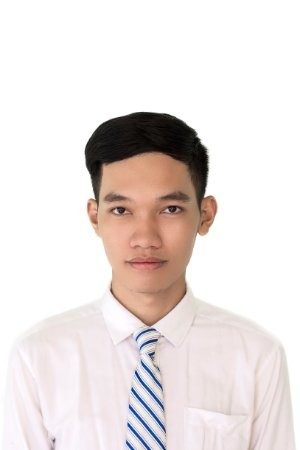
\includegraphics[scale=0.35]{picture}}
%\end{picture}
%-----       resume       ---------------------------------------------------------
\makecvtitle
\section{Education}
\cventry{2011-2016}{Undergraduate Degree}{University of Information Technology - VNU-HCM}{Ho Chi Minh City}{\textit{GPA: \textbf{9.02}/10}}
{Major: Computer Networks and Communications
\\ Thesis: "Build management and control system for surveillance cameras with Raspberry Pi"
\\ Advisor: Dr. Tuan \textsc{Nguyen-Anh} - Grade: \textbf{9.4}/10\\}  % arguments 3 to 6 can be left empty

\cventry{2016 - present}{Master's Degree}{University of Information Technology - VNU-HCM}{Ho Chi Minh City}{\textit{GPA: \textbf{8.97}/10}}{Major: Computer Science\\
Thesis: "An empirical study on DDoS detection and mitigation for Software-Defined
Networking" \\ Advisor: Dr. Van-Hau \textsc{Pham}}

\section{Research Interest and Objective}
\cvitem{Principal research interests}{\emph{future networks architecture, SDN, containerization, network security.}}
Earning a Bachelor's degree in Computer Networks and Communications, Hoa is currently pursuing a master's degree in Computer Science, which is the core of information technology to cultivate his knowledge in computer vision, machine learning, and distributed computing. 

He is seeking for an academic internship opportunity to leverage his expertise as well as his experiences to undertake postgraduate research regarding computer networks, especially in future network architectures, mobile computing and how to apply machine learning to networking, thus making a cornerstone preparation for the Ph.D. research afterward. 


\section{Experience}
\subsection{Research}
\begin{itemize}
	\item Working as a research assistant with a professor.
	\item Conducting a literature review, and self-research.
	\item Collecting dataset, conducting experiments and empirical research.
	\item Writing, publishing and presenting research papers.

\end{itemize}

\subsection{Teaching}
\begin{itemize}
	\item Teaching Assistant and Instructor for computer networks and information security courses:
	\begin{itemize}
		\item \textbf{Network courses:} \textit{Introduction to Computer Networks; Networks and Systems Administration; Basic Network Programming; Network-based and Web-based Application Development.}
		\item \textbf{Security courses:} \textit{Cryptography; Network security (Basic and Advanced courses); Personnel security, identification, and authentication; Ethical Hacking.}
	\end{itemize}
	\item CCNA Cisco Academy Instructor (CCAI) Certificate.	
\end{itemize}

\subsection{Leadership and Management}
\cventry{3/2015 -- 12/2015}{Vietnam National Union of Students (VNUS) in UIT}{Chairman}{UIT -- VNU-HCM}{}{
\begin{itemize}
	\item Captain of "Green Summer" Volunteer Campaign 2015.
	\item Head of organization of "UIT Student Leader" contest 2015.
\end{itemize}
}

\cventry{3/2017 -- present}{Youth Union of Faculty of Computer Networks and Communications, UIT}{Chairman}{UIT -- VNU-HCM}{}{
\begin{itemize}
	\item Head of organization of \textit{$1^{st}$ Security Day} and \textit{$1^{st}$ Network Day in UIT} (2017).
	\item Mentor of two \textit{Student Academic Club} about Information Security and Computer Networks .
\end{itemize}
}

\subsection{International activities}
\cventry{6/2014 - 7/2014}{Japan-East Asia Network of Exchange for Students and Youths}{Vietnam's member delegation}{Tokyo and Gifu, Japan}{}{}

\cventry{7/2015 - 8/2015}{"Green Summer" volunteer campain}{Leader of IT Team, Vietnam's member delegation}{Champasak, Laos}{}{Training statistical analysis (SPSS and R) for Champasak University lecturers}


\section{Techical Skills}
\begin{itemize}
  \item Programming languages: Python; PHP; HTML/CSS - Javascript; C++; C\#, Java.
  \item Software-Defined Networking (SDN): SDN Testbed, Ryu, OpenFlow, OpenvSwitch.
  \item Containerization \textit{(Docker, Kubernetes, Rancher)} and Vituarlization \textit{(VMWare)} techniques.
  \item Configuring Cisco network devices, next-gen firewalls (SOPHOS).
  \item Report: \LaTeX, Microsoft Office, Google Docs.
  \end{itemize}

\section{Languages}
\cvitemwithcomment{English}{Upper Intermediate}{TOEIC: Reading and Listening: 660/990; Speaking and Writing: 301/400}
\cvitemwithcomment{Vietnamese}{Mothertongue}{}

\section{Awards and Honors}
\begin{itemize}
	\item "\textit{Best Paper}" award in The $3^{rd}$ Symposium on Information Security (SoIS 2018, Vietnam).
	\item "\textit{Excellent staff}" award at UIT for two consecutive years in 2017 and 2018. 
	\item "\textit{Student of Five Merits}" award at National level in 2015. 
\end{itemize}

\section{References}
\begin{cvcolumns}
  \cvcolumn{Dr. Tuan \textsc{Nguyen-Anh}}{Vice Rector of UIT\\
  Email: \textit{tuanna@uit.edu.vn}}
  \cvcolumn{Dr. Van-Hau Pham}{Head of Information Security Lab, UIT\\
  Email: \textit{haupv@uit.edu.vn}}
  \cvcolumn[0.38]{Assoc. Prof. Quan Le-Trung}{Dean of Faculty of Computer Networks and Communications, UIT \\ Email: \textit{quanlt@uit.edu.vn}}
\end{cvcolumns}
% Publications from a BibTeX file without multibib
%  for numerical labels: \renewcommand{\bibliographyitemlabel}{\@biblabel{\arabic{enumiv}}}% CONSIDER MERGING WITH PREAMBLE PART
%  to redefine the heading string ("Publications"): \renewcommand{\refname}{Articles}
\nocite{*}
\bibliographystyle{plain}
\bibliography{publications}                        % 'publications' is the name of a BibTeX file
% Publications from a BibTeX file using the multibib package
%\section{Publications}
%\nocitebook{book1,book2}
%\bibliographystylebook{plain}
%\bibliographybook{publications}                   % 'publications' is the name of a BibTeX file
%\nocitemisc{misc1,misc2,misc3}
%\bibliographystylemisc{plain}
%\bibliographymisc{publications}                   % 'publications' is the name of a BibTeX file
\end{document}


%% end of file `template.tex'.